\ifx\allfiles\undefined
\documentclass[12pt, a4paper, oneside, UTF8]{ctexbook}
\def\path{../config}
\usepackage{amsmath}
\usepackage{amsthm}
\usepackage{amssymb}
\usepackage{array}
\usepackage{xcolor}
\usepackage{graphicx}
\usepackage{mathrsfs}
\usepackage{enumitem}
\usepackage{geometry}
\usepackage[colorlinks, linkcolor=black]{hyperref}
\usepackage{stackengine}
\usepackage{yhmath}
\usepackage{extarrows}
\usepackage{tikz}
\usepackage{pgfplots}
\usepackage{asymptote}
\usepackage{float}
\usepackage{fontspec} % 使用字体

\setmainfont{Times New Roman}
\setCJKmainfont{LXGWWenKai-Light}[
    SlantedFont=*
]

\everymath{\displaystyle}

\usepgfplotslibrary{polar}
\usepackage{subcaption}
\usetikzlibrary{decorations.pathreplacing, positioning}

\usepgfplotslibrary{fillbetween}
\pgfplotsset{compat=1.18}
% \usepackage{unicode-math}
\usepackage{esint}
\usepackage[most]{tcolorbox}

\usepackage{fancyhdr}
\usepackage[dvipsnames, svgnames]{xcolor}
\usepackage{listings}

\definecolor{mygreen}{rgb}{0,0.6,0}
\definecolor{mygray}{rgb}{0.5,0.5,0.5}
\definecolor{mymauve}{rgb}{0.58,0,0.82}
\definecolor{NavyBlue}{RGB}{0,0,128}
\definecolor{Rhodamine}{RGB}{255,0,255}
\definecolor{PineGreen}{RGB}{0,128,0}

\graphicspath{ {figures/},{../figures/}, {config/}, {../config/} }

\linespread{1.6}

\geometry{
    top=25.4mm, 
    bottom=25.4mm, 
    left=20mm, 
    right=20mm, 
    headheight=2.17cm, 
    headsep=4mm, 
    footskip=12mm
}

\setenumerate[1]{itemsep=5pt,partopsep=0pt,parsep=\parskip,topsep=5pt}
\setitemize[1]{itemsep=5pt,partopsep=0pt,parsep=\parskip,topsep=5pt}
\setdescription{itemsep=5pt,partopsep=0pt,parsep=\parskip,topsep=5pt}

\lstset{
    language=Mathematica,
    basicstyle=\tt,
    breaklines=true,
    keywordstyle=\bfseries\color{NavyBlue}, 
    emphstyle=\bfseries\color{Rhodamine},
    commentstyle=\itshape\color{black!50!white}, 
    stringstyle=\bfseries\color{PineGreen!90!black},
    columns=flexible,
    numbers=left,
    numberstyle=\footnotesize,
    frame=tb,
    breakatwhitespace=false,
} 

\lstset{
    language=TeX, % 设置语言为 TeX
    basicstyle=\ttfamily, % 使用等宽字体
    breaklines=true, % 自动换行
    keywordstyle=\bfseries\color{NavyBlue}, % 关键字样式
    emphstyle=\bfseries\color{Rhodamine}, % 强调样式
    commentstyle=\itshape\color{black!50!white}, % 注释样式
    stringstyle=\bfseries\color{PineGreen!90!black}, % 字符串样式
    columns=flexible, % 列的灵活性
    numbers=left, % 行号在左侧
    numberstyle=\footnotesize, % 行号字体大小
    frame=tb, % 顶部和底部边框
    breakatwhitespace=false % 不在空白处断行
}

% \begin{lstlisting}[language=TeX] ... \end{lstlisting}

% 定理环境设置
\usepackage[strict]{changepage} 
\usepackage{framed}

\definecolor{greenshade}{rgb}{0.90,1,0.92}
\definecolor{redshade}{rgb}{1.00,0.88,0.88}
\definecolor{brownshade}{rgb}{0.99,0.95,0.9}
\definecolor{lilacshade}{rgb}{0.95,0.93,0.98}
\definecolor{orangeshade}{rgb}{1.00,0.88,0.82}
\definecolor{lightblueshade}{rgb}{0.8,0.92,1}
\definecolor{purple}{rgb}{0.81,0.85,1}

\theoremstyle{definition}
\newtheorem{myDefn}{\indent Definition}[section]
\newtheorem{myLemma}{\indent Lemma}[section]
\newtheorem{myThm}[myLemma]{\indent Theorem}
\newtheorem{myCorollary}[myLemma]{\indent Corollary}
\newtheorem{myCriterion}[myLemma]{\indent Criterion}
\newtheorem*{myRemark}{\indent Remark}
\newtheorem{myProposition}{\indent Proposition}[section]

\newenvironment{formal}[2][]{%
	\def\FrameCommand{%
		\hspace{1pt}%
		{\color{#1}\vrule width 2pt}%
		{\color{#2}\vrule width 4pt}%
		\colorbox{#2}%
	}%
	\MakeFramed{\advance\hsize-\width\FrameRestore}%
	\noindent\hspace{-4.55pt}%
	\begin{adjustwidth}{}{7pt}\vspace{2pt}\vspace{2pt}}{%
		\vspace{2pt}\end{adjustwidth}\endMakeFramed%
}

\newenvironment{definition}{\vspace{-\baselineskip * 2 / 3}%
	\begin{formal}[Green]{greenshade}\vspace{-\baselineskip * 4 / 5}\begin{myDefn}}
	{\end{myDefn}\end{formal}\vspace{-\baselineskip * 2 / 3}}

\newenvironment{theorem}{\vspace{-\baselineskip * 2 / 3}%
	\begin{formal}[LightSkyBlue]{lightblueshade}\vspace{-\baselineskip * 4 / 5}\begin{myThm}}%
	{\end{myThm}\end{formal}\vspace{-\baselineskip * 2 / 3}}

\newenvironment{lemma}{\vspace{-\baselineskip * 2 / 3}%
	\begin{formal}[Plum]{lilacshade}\vspace{-\baselineskip * 4 / 5}\begin{myLemma}}%
	{\end{myLemma}\end{formal}\vspace{-\baselineskip * 2 / 3}}

\newenvironment{corollary}{\vspace{-\baselineskip * 2 / 3}%
	\begin{formal}[BurlyWood]{brownshade}\vspace{-\baselineskip * 4 / 5}\begin{myCorollary}}%
	{\end{myCorollary}\end{formal}\vspace{-\baselineskip * 2 / 3}}

\newenvironment{criterion}{\vspace{-\baselineskip * 2 / 3}%
	\begin{formal}[DarkOrange]{orangeshade}\vspace{-\baselineskip * 4 / 5}\begin{myCriterion}}%
	{\end{myCriterion}\end{formal}\vspace{-\baselineskip * 2 / 3}}
	

\newenvironment{remark}{\vspace{-\baselineskip * 2 / 3}%
	\begin{formal}[LightCoral]{redshade}\vspace{-\baselineskip * 4 / 5}\begin{myRemark}}%
	{\end{myRemark}\end{formal}\vspace{-\baselineskip * 2 / 3}}

\newenvironment{proposition}{\vspace{-\baselineskip * 2 / 3}%
	\begin{formal}[RoyalPurple]{purple}\vspace{-\baselineskip * 4 / 5}\begin{myProposition}}%
	{\end{myProposition}\end{formal}\vspace{-\baselineskip * 2 / 3}}


\newtheorem{example}{\indent \color{SeaGreen}{Example}}[section]
\renewcommand{\proofname}{\indent\textbf{\textcolor{TealBlue}{Proof}}}
\NewEnviron{solution}{%
	\begin{proof}[\indent\textbf{\textcolor{TealBlue}{Solution}}]%
		\color{blue}% 设置内容为蓝色
		\BODY% 插入环境内容
		\color{black}% 恢复默认颜色(可选,避免影响后续文字)
	\end{proof}%
}

% 自定义命令的文件

\def\d{\mathrm{d}}
\def\R{\mathbb{R}}
%\newcommand{\bs}[1]{\boldsymbol{#1}}
%\newcommand{\ora}[1]{\overrightarrow{#1}}
\newcommand{\myspace}[1]{\par\vspace{#1\baselineskip}}
\newcommand{\xrowht}[2][0]{\addstackgap[.5\dimexpr#2\relax]{\vphantom{#1}}}
\newenvironment{mycases}[1][1]{\linespread{#1} \selectfont \begin{cases}}{\end{cases}}
\newenvironment{myvmatrix}[1][1]{\linespread{#1} \selectfont \begin{vmatrix}}{\end{vmatrix}}
\newcommand{\tabincell}[2]{\begin{tabular}{@{}#1@{}}#2\end{tabular}}
\newcommand{\pll}{\kern 0.56em/\kern -0.8em /\kern 0.56em}
\newcommand{\dive}[1][F]{\mathrm{div}\;\boldsymbol{#1}}
\newcommand{\rotn}[1][A]{\mathrm{rot}\;\boldsymbol{#1}}

\newif\ifshowanswers
\showanswerstrue % 注释掉这行就不显示答案

% 定义答案环境
\newcommand{\answer}[1]{%
    \ifshowanswers
        #1%
    \fi
}

% 修改参数改变封面样式,0 默认原始封面、内置其他1、2、3种封面样式
\def\myIndex{0}


\ifnum\myIndex>0
    \input{\path/cover_package_\myIndex} 
\fi

\def\myTitle{考研数学笔记}
\def\myAuthor{Weary Bird}
\def\myDateCover{\today}
\def\myDateForeword{\today}
\def\myForeword{相见欢·林花谢了春红}
\def\myForewordText{
    林花谢了春红,太匆匆。
    无奈朝来寒雨晚来风。
    胭脂泪,相留醉,几时重。
    自是人生长恨水长东。
}
\def\mySubheading{以姜晓千强化课讲义为底本}


\begin{document}
% \input{\path/cover_text_\myIndex.tex}

\newpage
\thispagestyle{empty}
\begin{center}
    \Huge\textbf{\myForeword}
\end{center}
\myForewordText
\begin{flushright}
    \begin{tabular}{c}
        \myDateForeword
    \end{tabular}
\end{flushright}

\newpage
\pagestyle{plain}
\setcounter{page}{1}
\pagenumbering{Roman}
\tableofcontents

\newpage
\pagenumbering{arabic}
% \setcounter{chapter}{-1}
\setcounter{page}{1}

\pagestyle{fancy}
\fancyfoot[C]{\thepage}
\renewcommand{\headrulewidth}{0.4pt}
\renewcommand{\footrulewidth}{0pt}








\else
\fi
\chapter{操作系统}
\section{选择题}

\subsection{25-王道}
\begin{enumerate}
    \item 系统调用是由操作系统提供给用户的,它() \\
    A.直接通过键盘交互方式使用\qquad B.只能通过用户程序间接使用 \\
    C.是命令接口中的命令\qquad D.与系统的命令一样
    
    \item 操作系统与用户通信接口通常不包括() \\
    A.shell\qquad B.命令解释器\qquad C.广义指令\qquad D.缓存管理指令 

    \item 下列关于多道程序系统的叙述中,不正确的是() \\
    A.支持程序的并发执行\qquad B.不必支持虚拟存储管理 \\
    C.需要实现对共享资源的管理\qquad D.进程数越多CPU利用率也越多 

    \item 分时系统的一个重要指标是系统的响应时间,对操作系统的()因素改进有利于改善操作系统的响应时间. \\
    A.加大时间片\qquad B.采用静态页式管理 \\
    C.优先级+非抢占式调度算法\qquad D.代码可重入 

    \item 计算机区分内核态和用户态指令后,从核心态到用户态的转变用操作系统执行后完成,而用户态转换到核心态则有()完成 \\
    A. 硬件\qquad B.核心态程序\qquad C.用户程序\qquad D.中断处理程序

    \item "访管"指令()使用 \\
    A. 仅在用户态\qquad B.仅在内核态\qquad C.在规定时间内\qquad D.在调度时间内

    \item 在操作系统中,只能在核心态下执行的指令是() \\
    A. 读时钟\qquad B.取数\qquad C.广义指令\qquad D.寄存器清零

    \item \bt\bl 中断处理和子程序调用都需要压栈以保护现场,中断处理一定会保存而子程序调用不一定需要保存的内容是() \\
    A. 程序计数器\qquad B.程序状态字寄存器\qquad C.通用寄存器组\qquad D.通用地址寄存器

    \item \bt 定时器产生时钟中断后,由时钟中断服务程序更新的内容是()
    \begin{enumerate}
        \item [I] 内核中时间变量的值
        \item [II] 当前进程占用的CPU时间
        \item [III] 当前进程在时间片中的剩余执行时间
    \end{enumerate}
    A.仅I,II\qquad B.仅II,III\qquad C.仅I,III\qquad D.I,II,III

    \item \bt\bl 下列与中断相关的操作中,由操作系统完成的是(多选)()  
    \begin{enumerate}
        \item [I] 保存中断点
        \item [II] 提供中断服务
        \item [III] 初始化中断向量表
        \item [IV] 保存中断屏蔽字
    \end{enumerate}

    \item \bl 计算机的启动过程是(排序)() 
    \begin{enumerate}
        \item [1] CPU加点, CS:IP指向FFFF0H
        \item [2] 进行操作系统引导
        \item [3] 执行JMP指令跳转到BIOS
        \item [4] 登记BIOS中断例程入口地址
        \item [5] 硬件自检
    \end{enumerate}

    \item 在单处理机系统中,若同时存在10个进程,则处于就绪队列的进程最多有() \\
    A. 10个\qquad B.9个\qquad C.8个\qquad D.7个 

    \item 进程在处理器上执行时,() \\
    A. 进程之间是无关的,且具有封闭特性 \\
    B. 进程之间都有交互性,相互依赖,相互制约,具有并发性 \\
    C. 具有并发性,即同时执行的特性 \\
    D. 进程之间可能是无关的,但也可能是具有交互性的

    \item 在多对一的线程模型中,当一个多线程中的某线程被阻塞后() \\
    A. 该进程的其他线程仍然能够运行 \qquad B. 整个进程将被阻塞 \\
    C. 该阻塞进程将被撤销\qquad D. 该阻塞线程将永远不能再执行 

    \item 系统动态DLL库中的系统线程,被不同的进程所调用,它们是()的线程 \\
    A. 不同\qquad B.相同\qquad C.可能不同,可能相同\qquad D.不能被调用

    \item 下列不是多线程系统特长的是() \\
    A. 利用线程可以并发地执行矩阵乘法计算 \\
    B. Web服务器利用线程响应HTTP请求 \\
    C.键盘驱动程序为每个正在运行的程序配备一个线程,用以响应用户的输入 \\
    D. 基于GUI的调试程序用不同的线程分别处理用户输入,计算和跟踪等操作

    \item 下列选中,导致创建新进程的操作是(多选)() \\
    I.用户登录成功\qquad II.设备分配\qquad III,启动用户执行

    \item 可能导致进程被唤醒的事件是(多选)() \\
    I. I/O结束\qquad II.某进程退出临界区\qquad III.当前进程的时间片用完 

    \item 下列关于父进程与子进程的说法中错误的是() \\
    A.父进程和子进程可以并发执行 \\
    B.父进程和子进程共享虚拟地址空间 \\
    C.父进程和子进程有不同进程控制块 \\
    D.父进程和子进程共享临界资源

    \item 一个作业8:00到达系统,估计运行时间为1h,若10:00开始执行作业,其响应比为()

    \item 在进程调度算法中对短进程不利的是() \\
    A. 短进程优先调度\qquad B.先来先服务调度 \\
    C.高响应比优先调度算法\qquad D.多级反馈优先队列

    \item 不需要信号量就能实现的功能是() \\
    A.进程同步\qquad B.进程互斥\qquad C.进程的前驱关系\qquad D.进程的并发执行

    \item 若一个信号量的初始值为3,经过多次PV操作后当前值为-1,这表示进入临界区的进程数是() \\
    A. 1\qquad B.2\qquad C.3\qquad D.4

    \item 以下()属于临界资源 \\
    A. 打印机\qquad B.公用队列\qquad C.私有数据\qquad D.可重入的程序代码 

    \item 一个进程因在互斥信号量mutex上执行V操作而导致唤醒另一个进程的时,执行V操作后mutex的值为() \\
    A.大于0\qquad B.小于0\qquad C.大于等于0\qquad D.小于等于0 

    \item 进程P1和进程P2均包含并发执行的线程,部分伪代码如下,下列选项中,需要互斥执行的操作是() 
    \begin{center}
        \begin{minipage}[t]{0.45\textwidth}
\begin{lstlisting}[language=C]
// 进程P1                    
int x = 0;                   
Thread1() {                  
    int a;
    a = 1;
    x += 1;
}
Thread2() {
    int a;
    a = 2;
    x += 2;
}
\end{lstlisting}
        \end{minipage}
        \hfill
        \begin{minipage}[t]{0.45\textwidth}
\begin{lstlisting}[language=C]
// 进程P2                    
int x = 0;                   
Thread3() {                  
    int a;
    a = x;
    x += 3;
}
Thread4() {
    int a;
    b = x;
    x += 4;
}
\end{lstlisting}
        \end{minipage}
    \end{center}

    A.a=1与a=2\qquad B. a=x与b=x\qquad C.x +=1 与 x+=2\qquad D.x+=1与x+=3
    \item 下面是一个并发进程的程序代码,正确的是() 
    \begin{center}
        \begin{minipage}[t]{0.45\textwidth}
            \begin{lstlisting}[language=C]
Semaphore x1=x2=y=1;
int c1=c2=0;
P1() {
    while(1) {
        P(x1);
        if(++c1 == c) P(y);
        V(x1);
        computer(A);
        P(x1);
        if(--c1 == 0) V(y);
        V(x1);
    }
}
                \end{lstlisting}
            \end{minipage}
            \hfil
            \begin{minipage}[t]{0.45\textwidth}
                \begin{lstlisting}
Semaphore x1=x2=y=1;
int c1=c2=0;
P2() {
    while(1) {
        P(x2);
        if(++c2 == 1) P(y);
        V(x2);
        computer(B);
        P(x2);
        if(--c2 == 0) V(y);
        V(x2);
    }
}
            \end{lstlisting}
        \end{minipage}
    \end{center}
A.进程不会死锁,也不会饥饿 \qquad B.进程不会死锁,但会饥饿 \\
C.进程会死锁,但是不会饥饿\qquad D.进程会死锁,也会饥饿 

    \item 有两个并发进程,对于如这段程序的执行,正确的是() 
\begin{center}
    \begin{minipage}[t]{0.45\textwidth}
        \begin{lstlisting}
int x, y, z, t, u;
P1() {
    while(1) {
        x = 1;
        y = 0;
        if (x >= 1) y = y + 1;
        z = y;
    }
}
    \end{lstlisting}
\end{minipage}
\hfil
\begin{minipage}[t]{0.45\textwidth}
    \begin{lstlisting}
int x, y, z, t, u;
P2() {
    while(1) {
        x = 0;
        t = 0;
        if (x <= 1) t = t + 1;
        u = t;
    }
}
            \end{lstlisting}
        \end{minipage}
    \end{center}
    A.程序能够正常运行,结果唯一\qquad B.程序不能正常运行,可能出现两种结果\\
    C.程序不能正常运行,结果不确定\qquad D.程序不能正确运行,可能会死锁


    \item 若系统S1采用死锁避免方法,S2采用死锁检查方法,下列叙述中,正确的是(多选)() \\
    I. S1会限制用户申请资源的顺序,而S2不会 \\
    II. S1需要进程运行所需要的资源信息,而S2不需要 \\
    III. S1不会给可能导致死锁的进程分配资源,但S2会

    \item 下列存储管理方案中,()方式可以采用静态重定位 \\
    A.固定分区\qquad B.可变分区\qquad C.页式\qquad D.段式

    \item 下列不会产生内部碎片的存储管理是() \\
    A.分页式\qquad B.分段式\qquad C.段页式\qquad D.固定分区

    \item 采用分页和分段管理后,提供给用户的物理地址空间() \\
    A.分页支持更大的物理地址空间\qquad B.分段支持更大的物理地址空间 \\
    C.不能确定\qquad D.一样大

    \item 可重入程序是通过()方法来改善系统性能的. \\
    A.改变时间片长度\qquad B.改变用户数\qquad C.提供对换速度\qquad D.减少对换数量 

    \item 对主存储器的访问() \\
    A.以块(页)为单位 \qquad B.以字节或字位单位 \\
    C.随存储器的管理方案有所不同\qquad D.以用户的逻辑记录为单位

    \item 操作系统采用分页存储管理,要求() \\
    A.每个进程拥有一张页表,且进程的页表驻留在内存中 \\
    B.每个进程拥有一张页表,仅运行的进程的页表驻留在内存中\\
    C.所有进程共享一张页表,以节约有限的内存空间,但页表必须驻留在内存中 \\
    D.每个进程共享一张页表,只有页表中当前使用的页表必须驻留以最大限度节约有限的内存空间

    \item 在下列动态分区分配算法中,最容易产生内部碎片的是()  \\
    A.首次适应算法\qquad B.最坏适应算法\qquad C.最佳适应算法\qquad D.循环首次适应算法

    \item 请求分页存储管理中,若把页面尺寸增大一倍且可容纳的最大页数不变,则在程序顺序执行时缺页中断次数
    将会() \\
    A.增加\qquad B.减少\qquad C.不变\qquad D.无法确定

    \item 考虑页面置换算法,系统有m个物理块供调度,初始时全空,页面引用串长度为p,包含n个不同的页号,无论用啥算法
    缺页次数不会少于()

    \item 设主存容量为1MB,外存容量为400MB,计算机系统的地址寄存器有32位,那么虚拟存储器的最大容量是() 

    \item 导致LRU算法实现起来消耗特高的原因是() \\
    A.需要特殊硬件支持\qquad B.需要特殊的中断处理程序 \\
    C.需要在页表中标明特殊的页类型\qquad D.需要对所有页进行排序

    \item 在页面置换策略中,()策略可能引起抖动. 
    \begin{choices}
        \task FIFO
        \task LRU
        \task 没有一种 
        \task 所有 
    \end{choices}

    \item 提供虚拟存储技术的存储管理方法右() 
    \begin{choices}[2]
        \task 动态分区存储管理
        \task 页式存储管理
        \task 请求段式存储管理
        \task 存储覆盖技术
    \end{choices}

    \item 下列说法中正确的是() 
    \begin{enumerate}
        \item [(1)] 先进先出页面置换算法会产生Belady现象
        \item [(2)] 最近最少使用算法会产生Belady现象
        \item [(3)] 在进程运行时,若其工作集页面都在虚拟存储器内,则能够使该进程有效地进行,否则
        会频繁的页面调入/调出
        \item [(4)] 在进程运行时,若其工作集页面都在主存储器内,则能够使该进程有效地进行,否则
        会频繁的页面调入/调出
    \end{enumerate}
    \begin{choices}
        \task 1,3
        \task 1,4
        \task 2,3
        \task 2,4
    \end{choices}

    \item \bl 系统为某进程分配了4个页框,该进程已访问的页号序列为\underline{2,0,2,9,3,4,2,8,2,4,8.4.5}.
    若进程要访问的下一页的页号为7,依据LRU算法,应淘汰的页号是(   ) 

\end{enumerate}

\subsection{强化-1000题}
\begin{enumerate}
    \item 响应时间是衡量分时操作系统性能的重要指标,下列选项中,能够改善响应时间的是
    \begin{choices}[1]
    \task 允许用户修改系统时间
    \task 加大时间片
    \task 允许中断嵌套
    \task 采用抢占式优先级调度
    \end{choices}

    \item 下列选项中,能够引起内部中断的有\\
    I.除数为0\quad
    II.自陷指令\quad
    III.断电\quad
    IV.无效存储访问
    \begin{choices}[2]
    \task 仅I、II
    \task 仅II、III、IV
    \task 仅I、II、IV
    \task I、II、III、IV
    \end{choices}

    \item 下面关于时钟中断的说法,正确的说法个数是\\
    I.时钟中断的产生频率由硬件决定\\
    II.时钟中断属于程序性中断\\
    III.时钟中断时间间隔是计算机中的基本计时单位\\
    IV.时钟中断的处理可能引发进程调度
    \begin{choices}
    \task 1个
    \task 2个
    \task 3个
    \task 4个
    \end{choices}

    \item 下列关于操作系统提供的接口管理功能的叙述中,正确的是
    \begin{choices}[1]
    \task 联机用户接口用于多用户系统中各用户的交互与通信
    \task 脱机用户接口是为批处理作业的用户准备的,用户通过脱机用户接口与批处理作业进行交互
    \task 图形用户接口相比联机用户接口操作更方便,性能更优秀,运行图形界面耗费的资源也更少
    \task 程序接口是用户程序获得OS服务的唯一途径
    \end{choices}

    \item 下面关于中断、异常和系统调用的叙述中,正确的是
    \begin{choices}[1]
    \task 中断、异常和系统调用均可能发生在用户态或内核态
    \task 存在中断嵌套,但不存在系统调用嵌套
    \task 系统调用本质还是通过中断来实现的,一个OS的不同系统调用对应不同的中断入口
    \task 系统调用返回时,继续执行被调用程序
    \end{choices}

    \item 下列关于系统调用的说法中,正确的是\\
    I.当操作系统完成用户请求的“系统调用”功能后,应使CPU从内核态转到用户态工作\\
    II.用户程序设计时,使用系统调用命令,该命令经过编译后,形成若干参数和屏蔽中断指令\\
    III.用户在编写程序时计划读取某个数据文件中的20个数据块记录,需使用操作系统提供的系统调用接口\\
    IV.用户程序创建一个新进程,需使用操作系统提供的系统调用接口
    \begin{choices}[2]
    \task 仅I、III
    \task 仅II、IV
    \task 仅I、III、IV
    \task I、II、III、IV
    \end{choices}

    \item 下列操作中,可以在用户态执行的有\\
    I.执行除法指令\quad
    II.初始化中断向量表\quad
    III.执行Trap指令\\ 
    IV.从内存中取数\quad
    V.改变程序计数器(PC)的值\quad
    VI.关闭中断允许位
    \begin{choices}
    \task 2种
    \task 3种
    \task 4种
    \task 5种
    \end{choices}

    \item 静态重定位中,负责将指令中的逻辑地址转化为物理地址的是
    \begin{choices}
    \task 硬件
    \task 装入程序
    \task 用户程序
    \task 链接程序
    \end{choices}

    \item 下列关于操作系统结构的说法中,正确的是\\
    I.当前广泛使用的WindowsXP操作系统采用的是分层式OS结构\\
    II.模块化OS结构设计的基本原则是\ 每一层都仅使用其底层所提供的功能和服务,这样使系统的调试和验证都变得容易\\
    III.由于微内核结构能有效支持多处理机运行,故非常适合于分布式系统环境\\
    IV.采用微内核结构设计和实现操作系统具有诸多好处,如添加系统服务时不必修改内核,使系统更高效等
    \begin{choices}
    \task 仅I
    \task 仅I、III
    \task 仅III
    \task 仅III、IV
    \end{choices}

    \item 在计算机系统中,操作系统通常存储在()上,计算机开机后,操作系统最终被加载到
    \begin{choices}
    \task 硬盘:ROM
    \task BIOS:RAM
    \task 硬盘:RAM
    \task ROM:RAM
    \end{choices}

    \item 在计算机系统中,操作系统的引导程序一般存储在哪个区域?
    \begin{choices}
    \task 硬盘
    \task cache
    \task BIOS芯片
    \task 内存
    \end{choices}

    \item 下列关于虚拟机的说法正确的是\\
    I.第一类虚拟机的硬件资源的管理者是宿主操作系统\\
    II.第二类虚拟机的虚拟机管理程序负责把虚拟机程序的地址转换为内存中的物理地址\\
    III.第一类虚拟机的敏感指令不一定执行在内核态
    \begin{choices}
    \task I、II、III
    \task I、II
    \task II
    \task III
    \end{choices}

    \item 下列选项中,发生的事件和所导致的进程状态切换对应正确的有\\
    I. 当前进程时间片到期:执行→阻塞\\
    II. 当前进程申请临界资源:执行→就绪\\
    III. 当前进程的I/O操作结束:阻塞→就绪\\
    IV. 其他进程退出临界区:阻塞→就绪
    \begin{choices}
    \task 仅I、II
    \task 仅II
    \task 仅III、IV
    \task 仅II、III、IV
    \end{choices}

    \item 下列关于父子进程的说法中,正确的有\\
    I. 父进程和子进程内存空间相互独立\\
    II. 子进程先于父进程终止,子进程就会变成孤儿进程\\
    III. 父进程先于子进程终止,子进程就会变成僵尸进程\\
    IV. 父进程与子进程不能同时使用同一临界资源
    \begin{choices}
    \task 仅I、IV
    \task 仅II、III
    \task 仅I、II
    \task 仅II、III、IV
    \end{choices}

    % 15
    \item 在采用页式虚拟存储管理的操作系统中,进程P1在中断处理结束准备返回用户态的路径上触发调度,随后发生的进程切换中,哪些寄存器的内容一定需要保存?\\
    I. 页表基址寄存器\quad
    II. 栈顶指针寄存器\quad
    III. 程序计数器\quad
    IV. 栈基址寄存器\quad
    V. 通用寄存器
    \begin{choices}[2]
    \task I、II、III、V
    \task II、III、IV、V
    \task II、III、V
    \task I、II、III、IV、V
    \end{choices}


    \item 以下关于进程切换的说法中,正确的是
    \begin{choices}[1]
    \task 进程切换发生在用户态,从一个进程的运行态切换到另一个进程的运行态
    \task 中断/异常(系统调用)的发生是进程切换的前提
    \task 进程P0切换为进程P1的过程中,操作系统需要保存的信息有P1进程的断点、现场、堆栈中的数据、进程级打开文件表、P0进程的页表基址等信息
    \task 中断响应与进程切换保存和恢复上下文都是连续进行的
    \end{choices}


    \item 下列关于僵尸进程与孤儿进程的说法中,正确的有\\
    I. 子进程先于父进程退出,子进程就会变成僵尸进程\\
    II. 父进程先于子进程退出,子进程就会变成孤儿进程\\
    III. 僵尸进程有害\\
    IV. 孤儿进程无害
    \begin{choices}[2]
    \task 仅I、II
    \task 仅III、IV
    \task 仅I、II、III
    \task II、III、IV
    \end{choices}

    % 21
    \item 下列关于进程状态的转换的说法中,错误的是
    \begin{choices}[1]
    \task 进程状态的转换和对资源的需求都会记录在进程控制块中,进程结束时进程控制块需要回收
    \task 信号量的signal()和wait()操作其实是对系统调用的封装,会导致进程在运行态、就绪态和阻塞态之间转换
    \task 当进行进程调度时,一个高优先级的进程抢占低优先级进程的CPU后,低优先级进程的状态转为就绪态
    \task 成功执行完创建原语后,进程的状态转为创建态
    \end{choices}

    % 24
    \item 在支持多线程的操作系统中,有两种实现线程的方式:内核支持的线程和用户级线程。以下哪种说法是错误的?
    \begin{choices}[1]
    \task 用户级线程的上下文切换代价相对较小
    \task 内核支持的线程通常需要更多的内存空间来存储线程控制块和上下文信息,而用户级线程只需要存储少量的信息
    \task 内核支持的线程能够实现更好的多核性能和负载均衡并且公平性更好
    \task 用户级线程的调度由用户空间运行时系统完成,与操作系统无关
    \end{choices}


    \item 将内核支持线程(KST)与用户级线程(ULT)进行组合,可以实现组合方式的ULT/KST线程。下列关于多线程模型,说法错误的是
    \begin{choices}[1]
    \task 组合方式中,一些KST对应多个ULT,这是ULT通过时分多路复用KST来实现的
    \task 多对一模型与一对一模型相比,多对一模型的线程管理的开销小,效率高,一对一模型的并发性能更好
    \task 多对一模型中多个线程不能同时在多个处理机上运行;一对一模型中允许多个线程并行地在多处理机系统上运行
    \task 多对对模型中, KST数目可以比ULT数目少,也可以多余或者等于ULT数量
    \end{choices}


    \item 在现代多线程操作系统中,一个进程P首先创建了一个主线程T0。线程T0在执行过程中通过系统调用打开了一个网络套接字,并获得了对应的套接字描述符sockfd。随后,线程T0创建了两个新的子线程Ta和Tb来分别处理该套接字上的数据接收和发送。下列各项中,哪些是线程Ta和Tb可以共享的资源或信息?\\
    I. 进程P的全局变量\quad
    II. 线程T0的局部变量存储区域\\
    III. 套接字描述符sockfd\quad
    IV. 线程Ta和Tb各自独立的程序计数器
    \begin{choices}[2]
    \task 仅I、III
    \task 仅I、IV
    \task 仅I、III、IV
    \task I、II、III、IV
    \end{choices}


    \item 下列关于进程虚拟地址空间的说法中,错误的是
    \begin{choices}[1]
    \task 进程虚拟地址空间分为内核空间和用户空间,当CPU处于用户态时只能访问用户空间,处于内核态时可以访问内核空间和用户空间
    \task 每个进程的虚拟地址空间中,内核空间部分映射到相同的物理内存区域,即操作系统的代码和全局数据
    \task 每个进程都共享内核空间的同一份内核栈,用于保存内核处理中断/异常(系统调用)时的局部变量、返回地址等信息
    \task 当进程想要访问内核空间时,可以通过中断/异常(系统调用)进入内核态
    \end{choices}


    \item 下列关于管道(Pipe)通信的叙述中,错误的是
    \begin{choices}[1]
    \task 管道通常用于具有亲缘关系的进程(如父子进程)之间进行单向数据流通信
    \task 管道的实质是在内存中开辟的一个固定大小的缓冲区,其容量通常有限,并非无限大
    \task 当写进程向已满的管道中写入数据时,或者读进程从空管道中读取数据时,对应的进程将会被阻塞
    \task 管道位于进程的用户空间之中,可直接在用户态下读管道
    \end{choices}


    \item 一个管程中包含条件变量x,下面关于x的说法,错误的是
    \begin{choices}[1]
    \task x.signal()操作不一定会唤醒一个进程
    \task x.wait()操作不一定会阻塞一个进程
    \task x中通常拥有一个特定的阻塞队列
    \task 管程中定义x时,不需要对其进行初始化操作
    \end{choices}


    \item 下列关于管道(Pipe)通信的叙述中,正确的是
    \begin{choices}[1]
    \task 在利用管道文件通信时,可以使用操作系统为文件提供的一套系统调用接口,如open()、write()、read()、close()等
    \task 当所有引用管道的文件描述符都被关闭后,管道内未被读取完的数据会被持久化到磁盘之中
    \task 父进程在创建了管道之后又创建了两个子进程,子进程之间利用管道进行通信,当父进程被撤销时,这两个子进程之间的管道也被内核撤销
    \task 管道通信是以消息为单位进行写入和读出的
    \end{choices}


    \item 信号(Signal)是UNIX及类UNIX系统中一种重要的异步进程间通信方式。下列关于信号机制的叙述中,错误的是
    \begin{choices}[1]
    \task 信号可以由一个进程发送给另一个进程,也可以由内核发送给某个进程,甚至进程也可以给自身发信号
    \task 进程接收到信号后,可以忽略该信号、执行系统默认操作或执行用户自定义的处理函数
    \task 信号是一种轻量级的通信方式,适合用于传递大量复杂的数据结构
    \task 某些特定信号具有特殊含义,其默认行为不能被用户进程捕获或忽略
    \end{choices}


    \item 使用共享文件进行通信的方式属于()通信
    \begin{choices}[2]
    \task 共享存储
    \task 信号量
    \task 消息缓冲
    \task 管道
    \end{choices}


    \item 将数据由P1→P2→P3顺序传递,以下哪种进程通信机制最适合满足这个需求?
    \begin{choices}[2]
    \task 管道
    \task 消息队列
    \task 共享内存
    \task 信号量
    \end{choices}

    % 51-2
    \item 高性能计算服务器多进程应用工作模式如下所述,
    \begin{enumerate}
        \item[a.] 一个主进程P0与另一个无亲缘关系的主进程P1通信完毕后,从磁盘读取一个大型数据集(>1GB),并
        将其分割成多个数据块.
        \item[b.] 主进程P0创建多个子进程($P_a,P_b,\ldots,P_z$),并将这些数据块分发给子进程进行并行处理,这些子进程
        需要频繁,快速地读这些数据块
        \item [c.] 各子进程在处理完成后, 需要向主进程发送一条简短的完成信息 
        \item [d.] 任意子进程在遇到无法恢复的错误的时候,必须立即向主进程发送一个紧急的异常通知,主进程在收到通知后立刻中断当前
        工作并进行处理. 
    \end{enumerate}
    下列叙述中正确的是\\
    I. 步骤a中采用匿名管道的方式可以得到最高效率\\
    II. 步骤b中采用共享内存的方式可以获得最高效率\\
    III. 步骤c中采用消息传递的方式可以获得最高效率\\
    IV. 步骤d中采用信号的方式可以获得最高效率
    \begin{choices}[2]
    \task I、II
    \task I、III
    \task II、III
    \task II、IV
    \end{choices}


    \item 下列关于进程通信的叙述中,正确的有\\
    I. PV操作(信号量)、管程也可用于进程通信\\
    II. 共享内存是速度最快的通信方式\\
    III. 消息传递是当前应用最广泛的通信方式\\
    IV. 信号通信其实是一种软件中断
    \begin{choices}[2]
    \task 仅I、II、III
    \task 仅II、III、IV
    \task 仅I、III、IV
    \task I、II、III、IV
    \end{choices}


    \item 下列关于闲逛进程的说法中,错误的是
    \begin{choices}[1]
    \task 闲逛进程的优先级通常设置为最低,一旦有其他进程需要CPU资源,闲逛进程会立即让出CPU,让其他进程执行
    \task 大多数情况下,闲逛进程仅执行一个空循环,不执行任何实际操作
    \task 闲逛进程一般来说运行在用户态下
    \task 闲逛进程的进程转换只有运行态→就绪态和就绪态→运行态
    \end{choices}


    \item 高响应比优先的进程调度算法综合考虑了进程的等待时间和计算时间,响应比的定义是
    \begin{choices}[1]
    \task 进程周转时间与等待时间之比
    \task 进程周转时间与要求服务时间之比
    \task 进程等待时间与要求服务时间之比
    \task 要求服务时间与等待时间之比
    \end{choices}

    % 65
    \item 下列调度算法中,不宜设计为抢占式调度的是
    \begin{choices}[1]
    \task 时间片轮转
    \task 优先级
    \task 高响应比优先
    \task 多级反馈队列调度算法
    \end{choices}

    % 74
    \item 有3个作业: A(到达时间8:45,执行时间1.5 h),B(到达时间9:00,执行时间0.5 h),C(到达时间9:30,执行时间0.5 h)。当9:30作业全部到达后,操作系统按照非抢占式高响应比优先调度算法进行调度,则作业被选中执行的顺序是
    \begin{choices}[2]
    \task (A,B,C)
    \task (B,A,C)
    \task (B,C,A)
    \task (C,B,A)
    \end{choices}

    % 75
    \item 考虑在单纯时间片轮转算法中实现“优先级调度”,即优先级越高的进程一次分配的时间片越多。有进程A、B、C、D、E依次几乎同时到达,其预计运行时间分别为10、6、2、4、8,其优先级数分别是3、5、2、1、4,一个优先级数对应一个时间片。对于前一个进程时间片有剩余的情况,操作系统会调度下一个进程运行。这种情况下总周转时间是
    \begin{choices}
    \task 92
    \task 102
    \task 112
    \task 122
    \end{choices}

    % 83
    \item 下列关于SMP系统中处理器调度及其相关概念的叙述中,错误的是
    \begin{choices}[1]
    \task 自调度方式下,系统中通常维护一个所有处理器共享的全局就绪队列,空闲的处理器会主动从该队列中获取任务执行
    \task 成组调度策略倾向于将一个应用程序中的多个相关线程或进程组在同一时间分配到不同处理器上并行执行,以减少它们之间的同步等待开销
    \task 动态分配方式下,一个进程或线程在其生命周期内可能会被分配到不同的处理器上执行,这有助于实现负载均衡,但也可能降低高速缓存的命中率
    \task 专用处理器分配策略为每个就绪线程都分配一个独立的处理器,能最大限度地提高单个应用程序的并行度,且在任何情况下都能获得最佳的系统整体性能
    \end{choices}

    % 84
    \item 下列内容中,属于进程上下文的是\\
    I. 虚拟地址空间\quad
    II. PC的值\quad
    III. PSW寄存器的值\quad
    IV. 系统内核栈
    \begin{choices}[2]
    \task I、III
    \task I、IV
    \task I、II、III
    \task I、II、III、IV
    \end{choices}

    % 90
    \item 下列选项中,对于多个进程之间的同步与互斥,属于临界资源的是\\
    I. 打印机\quad
    II. 各进程的非共享数据\quad
    III. 磁盘\quad
    IV. 共享缓冲区
    \begin{choices}[2]
    \task 仅I、II
    \task 仅I、IV
    \task 仅I、II、IV
    \task I、II、III、IV
    \end{choices}

    % 95
    \item 进程P0和P1访问临界资源的伪代码实现如下,以下说法正确的是
    \begin{lstlisting}[language=C]
    bool flag[2]={false, false};
    // P0               
    while(flag[1]); // 进入区
    flag[0] = true; // 进入区
    critical section; // 临界区
    flag[0] = false; // 退出区
    remainder section; // 剩余区

    // P1 
    while(flag[0]);
    flag[1] = true;
    critical section;
    flag[1] = false;
    remainder section;
    \end{lstlisting}
    \begin{choices}[1]
    \task 不能保证进程互斥进入临界区,且违背了忙则等待原则
    \task 不能保证进程互斥进入临界区,但是遵循忙则等待原则
    \task 能保证进程互斥进入临界区,但是违背了忙则等待原则
    \task 能保证进程互斥进入临界区,且遵循忙则等待原则
    \end{choices}

    % 97
    \item 互斥锁是一种用于解决临界区互斥问题的常用手段,对acquire()获取锁或release()释放锁的调用必须原子地执行,因此,互斥锁通常采用硬件原语(如Test\&Set指令或exchange交换指令)来实现。对于TSL硬件原语实现的自旋锁与无忙等待锁,以下说法错误的是
    \begin{choices}[1]
    \task 使用原子操作指令实现的互斥锁适用于单处理器或共享内存多处理器中任意数量的进程同步
    \task 自旋锁不能实现让权等待,但是阻塞锁可以
    \task 自旋锁可以实现进程对临界区的先进先出(即按申请顺序访问临界区),不会导致进程饥饿
    \task 互斥锁可用于多进(线)程之间,但是只能由获取锁的进(线)程对它进行解锁(即释放)
    \end{choices}

    % 101
    \item 对记录型信号量S执行相关操作后,下列描述中正确的是\\
    I. 执行P操作时,当S.value<0时,阻塞当前进程\\
    II. 执行P操作时,当S.value≤0时,阻塞当前进程\\
    III. 执行V操作时,当S.value≤0时,唤醒一个阻塞队列进程\\
    IV. 执行V操作时,当S.value<0时,唤醒一个阻塞队列进程
    \begin{choices}[2]
    \task I、IV
    \task II、III
    \task I、III
    \task II、IV
    \end{choices}

    % 105
    \item 以下关于同步互斥的各种实现方法中,说法错误的是
    \begin{choices}[1]
    \task 禁用中断不可以在多处理机系统上实现同步原语
    \task 软件方法如Peterson,以及原子操作指令(TSL指令和SWAP指令)这些方法都不能实现让权等待
    \task 互斥锁无法实现让权等待,属于忙等机制
    \task 在管程中对条件变量执行signal操作时,如果该条件变量对应的等待队列为空,则丢弃该信号执行空操作
    \end{choices}

    % 111
    \item 以下关于进程死锁的表述,正确的有\\
    I. 如果每个进程只能拥有一个资源,则死锁就不会发生\\
    II. 如果所有资源多个进程都可以无冲突共享访问,则死锁就不会发生\\
    III. 如果所有进程的执行严格区分优先级,则死锁就不会发生\\
    IV. 如果进程资源请求之间不存在循环等待,则死锁就不会发生
    \begin{choices}[2]
    \task 仅I、II
    \task 仅II、IV
    \task 仅I、II、IV
    \task 仅II、III、IV
    \end{choices}

    % 116
    \item 下列关于死锁与安全状态的叙述中,错误的是\\
    I. 安全一定不死锁\\
    II. 死锁一定不安全\\
    III. 不安全必定会死锁\\
    IV. 不死锁一定处于安全状态
    \begin{choices}[2]
    \task 仅I、II
    \task 仅II、IV
    \task 仅I、IV
    \task 仅II、III
    \end{choices}

    % 118
    \item 两个进程A和B,每一个进程都需要申请资源1、2、3各一个,在系统中三种资源各只有一个。假如这两个进程都以1、2、3的次序申请,系统将不会发生死锁。但如果A以3、2、1的次序申请,B以1、2、3的次序申请,则死锁可能发生。两个进程申请资源的顺序如果不确定,那么系统保证不发生死锁的概率是
    \begin{choices}
    \task 1/9
    \task 1/6
    \task 1/3
    \task 1/12
    \end{choices}

    % 126
    \item 下列关于死锁解除策略的叙述中,错误的是
    \begin{choices}[1]
    \task 最简单直接的死锁解除方法是强制终止系统中的所有死锁进程,但这可能导致已完成大量工作的进程前功尽弃
    \task 采用“进程回退”策略时,系统将使一个或多个死锁进程回退到足以避免死锁的某个先前状态(检查点),但这要求系统记录进程的历史状态信息
    \task 剥夺资源是常用的死锁解除方法之一,即从一个或多个死锁进程中抢占某些资源,并将这些资源分配给其他死锁进程,但选择剥夺哪些资源和哪个进程的资源是一个复杂的问题
    \task 终止死锁进程时,选择优先级最低的死锁进程予以终止,可以保证系统为解除死锁付出的代价最小
    \end{choices}

    % 127
    \item 某系统有m个同类资源供n个进程共享,若每个进程最多申请k个资源(k>1),采用银行家算法分配资源,为保证系统不发生死锁,则各进程的最大需求量之和应
    \begin{choices}[2]
    \task 等于m
    \task 等于m+n
    \task 小于m+n
    \task 大于m+n
    \end{choices}

    % 128
    \item 下列关于死锁的预防、避免、检测和解除的叙述中,正确的有\\
    I. 资源的有序分配策略可以破坏死锁的请求和保持条件\\
    II. 银行家算法通过控制资源的分配,破坏了死锁的循环等待条件\\
    III. 产生死锁的根本原因是系统资源分配不足和进程推进顺序非法\\
    IV. 采用进程回退法解除死锁需要保存进程的历史信息,设置还原点
    \begin{choices}[2]
    \task 仅I、II
    \task 仅III、IV
    \task 仅II、III、IV
    \task I、II、III、IV
    \end{choices}

    % 6
    \item 在下列存储管理方式中,会产生内部碎片的是\\
    I. 分段虚拟存储管理\quad
    II. 分页虚拟存储管理\quad
    III. 段页式分区管理\quad
    IV. 固定式分区管理
    \begin{choices}[2]
    \task 仅II
    \task 仅III、IV
    \task 仅I、II、III
    \task 仅II、III、IV
    \end{choices}

    % 7
    \item 下列内存分配存储管理方式中,不会产生外部碎片的是
    \begin{choices}[1]
    \task 动态重定位分区分配
    \task 分页存储管理
    \task 可变分区分配
    \task 分段存储管理
    \end{choices}

    % 15
    \item 某台计算机采用动态分区来分配内存,经过一段时间的运行后,内存中按地址从小到大存在100\,KB、450\,KB、250\,KB、200\,KB和600\,KB的空闲分区。分配指针现在指向地址起始点,继续运行还会有212\,KB、417\,KB、112\,KB和426\,KB的进程申请使用内存,则能够完全完成分配任务的算法是
    \begin{choices}[2]
    \task 首次适应算法
    \task 邻近适应算法
    \task 最佳适应算法
    \task 最坏适应算法
    \end{choices}

    % 20
    \item 采用二级页表的分页系统中,一级页表页表项中的内容是
    \begin{choices}[2]
    \task 用于二级页表索引的页号
    \task 对应二级页表所在的页框号
    \task 页目录号
    \task 程序文件所在的页框号
    \end{choices}

    % 24
    \item 在一台以字节为单位寻址的64位计算机系统中,地址线宽为64位,实际使用的虚拟地址空间大小是256\,TB。若采用虚拟页式存储管理,每页的大小为8\,KB,页表表项长为8\,B,采用多级页表进行管理,则多级页表的级次最小是
    \begin{choices}
    \task 3
    \task 4
    \task 5
    \task 6
    \end{choices}

    % 27
    \item 系统按字节编址,采用请求分页存储方式管理内存,系统的逻辑地址空间大小为256\,TB,页面大小为8\,KB,页表项大小为8\,B,则该系统页表的级数应当是
    \begin{choices}
    \task 3
    \task 4
    \task 5
    \task 6
    \end{choices}

    
    \item 在采用分页存储管理的系统中,地址结构长度为18位,其中11至17位表示页号,0至10位表示页内偏移量,则主存容量最大可为()KB,主存可分为()个块。若有一作业依次被放入2、3、7号物理块,相对地址1500处有一条指令“store1,12500”,那么,该指令地址所在页的页号为0,指令的物理地址为(),该指令数据的存储地址所在页的页号为()。
    \begin{choices}[1]
    \task 256、256、5596、7
    \task 256、128、500、7
    \task 256、128、5596、6
    \task 256、128、5500、6
    \end{choices}


    \item 在支持虚拟内存的操作系统中,交换区(对换区,Swap Space)扮演着重要的角色。下列关于交换区的叙述中,错误的是\\
    I. 交换区是磁盘上的一块专用空间,用于存放从内存中换出的暂时不活跃的页面或整个进程\\
    II. 操作系统管理交换区时,通常会采用与管理文件系统类似的数据结构和分配策略,以实现灵活的空间管理\\
    III. 当物理内存不足时,操作系统可以将某些进程或进程的部分页面移至交换区,以释放物理内存给更需要的进程\\
    IV. 增大交换区的大小可以加快虚实地址的转换,从而提高虚拟内存管理的效率
    \begin{choices}[1]
    \task 仅I、II
    \task 仅II、III
    \task 仅II、IV
    \task 仅IV
    \end{choices}

    % 46
    \item 在请求分页管理中,已修改过的页面再次装入时应来自
    \begin{choices}[1]
    \task 磁盘文件区
    \task 磁盘对换区
    \task 后备作业区
    \task I/O缓冲区
    \end{choices}

    % 48
    \item 系统采用页式虚拟存储管理和固定分配局部置换策略,页框大小为512\,B,某个进程中有如下代码段。假设系统数组按行优先存放,为每个int型数据分配4\,B空间,该段代码已在内存,但要处理的数据不在内存,系统为该进程分配的数据区只有1个页框,则执行上述代码会发生()次缺页中断。(页面置换时不置换代码段所在页面)
    \begin{lstlisting}[language=C]
    int a[128][128];
    for (int i = 0; i < 128; i++)
        for (int j = 0; j < 128; j++)
            a[j][i] = 0;
    \end{lstlisting}
    \begin{choices}[1]
    \task 1
    \task 2
    \task 128
    \task 16384
    \end{choices}

    % 49
    \item 某分页虚拟存储管理系统中内存存取时间为1\,\textmu s。在处理缺页中断时,若还有可用的空页框或被替换的页未被修改,则处理一个缺页中断需要1\,ms;如果被替换的页已被修改,则处理一个缺页中断需要10\,ms。假定60\%的替换页被修改过,为保证有效存取时间不超过3\,\textmu s,可接受的最大缺页率是
    \begin{choices}[1]
    \task 1/164
    \task 1/64
    \task 1/16400
    \task 1/6400
    \end{choices}

    % 50
    \item 某计算机系统按字节编址,采用请求分页式存储管理方式,无TLB,访问一次内存需100\,\textmu s。在系统发生缺页中断时,若不需要调出页面或调出页面未被修改不需要写回磁盘,则缺页处理需要8.5\,ms;若调出页面被修改过,需要写回磁盘,则缺页处理需要21\,ms。缺页处理结束后,重新访问内存中的页表。若系统中有80\%的页面被修改过,要保证平均访存时间不超过386\,\textmu s,则缺页率不可以超过
    \begin{choices}[1]
    \task 1\%
    \task 1.5\%
    \task 2\%
    \task 5\%
    \end{choices}

    % 51
    \item 假设某系统中的TLB的命中率大约是75\%,并且使用了二级页表,则平均访存次数是(访问TLB的时间忽略)
    \begin{choices}[1]
    \task 平均需要1.25次内存访问
    \task 平均需要1.5次内存访问
    \task 平均需要1.75次内存访问
    \task 平均需要2次内存访问
    \end{choices}

    % 55
    \item 下列关于LRU算法及其近似算法硬件支持或实现方式的叙述中,错误的是
    \begin{choices}[1]
    \task 可以为每个物理页框设置一个移位寄存器,并周期性地右移,访问时将最高位置1,具有最小寄存器值的页面即为最近最久未使用页
    \task 可以利用一个特殊的硬件栈来维护当前在内存中页面的访问顺序,栈顶始终是最新访问的页面,栈底则是最近最久未使用的页面
    \task 操作系统可以通过在页表项中增加一个“访问位”,并周期性地清零该位,结合一个替换指针循环扫描来近似实现LRU算法
    \task 为了精确实现LRU,最简单且开销最小的方法是为每个页表项设置一个时间戳寄存器,记录该页最后一次被访问的精确系统时间
    \end{choices}

    % 57
    \item 页面置换算法LRU-K是LRU算法的变种,K代表最近使用的次数,LRU可以认为是LRU-1。下面介绍LRU-2算法,LRU-2算法需要维护两个队列(历史访问队列,缓存队列),需要访问某一页时,先查找缓存队列。①如果该页在缓存队列中,则可以直接访问,并且将该页重新放在缓存队列队尾位置。②如果该页未在缓存队列中但是在历史访问队列中,则将该页从历史访问队列移出并加入缓存队列中。③如果该页未在缓存队列且未在历史访问队列中,则该页放入历史访问队列并访问该页。假设两个队列长度都为5,队列采用FIFO淘汰策略,初始内存中没有数据,使用LRU-2算法,页号访问序列为:(5,6,7,8,3,8,5,9,6,8,3,4,7,5,6)。当第10次访问,访问到8号页时,缓存队列的队头是
    \begin{choices}[1]
    \task 3
    \task 5
    \task 8
    \task 6
    \end{choices}

    % 64
    \item 以下对置换算法和抖动的描述中正确的有\\
    I. 使用时钟(CLOCK)置换算法可能会产生Belady现象\\
    II. 使用先进先出(FIFO)页面置换算法可能会产生Belady现象\\
    III. 如果进程的工作集都被调入到了物理内存中,则进程的缺页率可以保持一个较低水平,否则会出现抖动现象\\
    IV. 如果进程的工作集都被调入到了虚拟内存中,则进程的缺页率可以保持一个较低水平,否则会出现抖动现象
    \begin{choices}[1]
    \task I、III
    \task I、IV
    \task I、II、III
    \task I、II、IV
    \end{choices}

    % 65
    \item 进程A在t时刻前访问了如下页面:3、6、3、4、9、5、9,在接下来的一段时间里还将访问页面:2、4、6、4、8、9。设工作集窗口大小为4,则进程A在t时刻时的工作集是
    \begin{choices}[1]
    \task 4、5、9
    \task 3、4、5、9
    \task 2、4、6、8
    \task 2、4、6
    \end{choices}

    % 66
    \item 在页式虚拟管理系统中,假定驻留集为m个页帧(初始所有页帧均为空),在长为p的引用串中具有n个不同页号(n>m),对于FIFO、LRU两种页面替换算法,其缺页中断的次数的范围分别为
    \begin{choices}[2]
    \task[A] [m,p]和[n,p]
    \task[B] [m,n]和[n,p]
    \task[C] [n,p]和[m,n]
    \task[D] [n,p]和[n,p]
    \end{choices}

    % 67
    \item 内存映射文件(Memory-Mapped File)是一种允许进程将文件内容直接映射到其虚拟地址空间的技术。下列关于内存映射文件的叙述中,错误的是
    \begin{choices}[1]
    \task 进程访问内存映射文件区域就像访问普通内存一样,无需显式的read()或write()系统调用
    \task 多个不同进程可以将同一个文件映射到它们各自的虚拟地址空间中,从而实现对该文件内容的高效共享
    \task 当一个进程修改其内存映射文件区域时,所做的修改会立即写回磁盘上的原始文件
    \task 内存映射文件区域的读写操作可能会引发缺页中断,操作系统会负责将文件内容从磁盘按需调入物理内存
    \end{choices}

    % 68
    \item 以下关于内存映射文件的说法中正确的有\\
    I. 一般的I/O操作中,从磁盘调入的文件会先写入内核的页高速缓存,然后再从页高速缓存复制到用户进程的缓冲区;而内存映射文件避免这次从内核空间到用户空间的额外数据复制,从而提高I/O效率\\
    II. 内存映射文件实现了从进程对应磁盘文件到其虚拟内存空间中某部分的映射\\
    III. 内存映射文件能为不同进程提供一个高带宽的通信通道\\
    IV. 进程通过系统调用将文件映射到其虚拟内存空间的一部分,并将这一文件全部调入到物理内存
    \begin{choices}[1]
    \task 仅I、II
    \task I、II、III
    \task I、III、IV
    \task I、II、III、IV
    \end{choices}

    % 69
    \item 下列选项中,能够影响系统缺页率的有\\
    I. 页面置换算法\quad
    II. 工作集的大小\quad
    III. 进程的数量\quad
    IV. 页缓冲队列的长度\quad
    V. 程序的编制方法
    \begin{choices}[1]
    \task I、II、III、V
    \task I、II、IV、V
    \task II、III、IV、V
    \task I、II、III、IV
    \end{choices}

    \item 关于I/O接口的I/O逻辑说法错误的是(\qquad)
    \begin{choices}[1]
    \task 不同I/O接口的I/O端口不重复,各I/O逻辑同时对地址线上的地址进行译码,分辨出此次传输是否属于自己
    \task 通过控制线的读/写信号来对地址标明的I/O端口进行读写
    \task 对控制寄存器的I/O命令字进行译码,对外设发出具体的控制
    \task 采集外设的状态,并通过控制线向CPU反馈设备状态信息以及发出中断请求
    \end{choices}

    \item 在下列关于各种I/O控制方式的说法中,错误的是(\qquad)
    \begin{choices}[1]
    \task 程序直接控制I/O方式适用于结构简单、只需少量硬件的电路,不需要设备驱动程序来完成数据的传输工作
    \task 中断驱动I/O方式适用于具有中断机构的系统,用于处理中低速的I/O操作和随机事件
    \task DMA方式适用于具有DMA控制器的系统,用于高速外设的大批量数据传输
    \task 设备驱动程序和各种I/O控制方式之间密切相关
    \end{choices}

    \item 键盘硬件产生输入后,系统的正确处理流程是(\qquad)
    \begin{choices}[1]
    \task 键盘硬件→中断处理程序→设备驱动程序→进程调度→系统调用返回→用户程序
    \task 键盘硬件→设备驱动程序→中断处理程序→系统调用返回→进程调度→用户程序
    \task 键盘硬件→系统调用返回→设备驱动程序→中断处理程序→进程调度→用户程序
    \task 键盘硬件→中断处理程序→系统调用返回→设备驱动程序→进程调度→用户程序
    \end{choices}

    \item 用户进程调用了读磁盘系统调用,其中将逻辑盘块号转换为物理地址的工作是由(\qquad)完成的
    \begin{choices}
    \task 设备无关软件
    \task 设备驱动程序
    \task 中断处理程序
    \task 硬件
    \end{choices}

    \item 以下设备管理工作中,适合由设备独立性软件来完成的有(\qquad)\\
    I.向控制寄存器写命令\quad
    II.检查用户是否有权使用设备\quad
    III.检查用户I/O请求的合法性\quad
    IV.缓冲管理
    \begin{choices}[2]
    \task I、II、III
    \task II、III、IV
    \task II、IV
    \task I、II、III、IV
    \end{choices}

    \item 设备分配策略与(\qquad)因素有关\\
    I.I/O设备的固有属性\quad
    II.系统所采用的分配策略\quad
    III.设备分配中的安全性\quad
    IV.设备的无关性
    \begin{choices}[2]
    \task I、II、III
    \task I、III、IV
    \task I、II、IV
    \task I、II、III、IV
    \end{choices}

    \item 设备分配策略的主要目标是(\qquad)\\
    I.确保设备不被过度使用\quad
    II.提高设备利用率\quad
    III.减少用户等待时间
    \begin{choices}[2]
    \task I、II
    \task I、III
    \task II、III
    \task I、II、III
    \end{choices}

    \item 在设备分配与回收过程中,计算机需要访问的数据结构有:设备控制表DCT、控制器控制表COCT、通道控制表CHCT和系统设备表SDT,它们在设备分配流程中访问的先后顺序为(\qquad)
    \begin{choices}[2]
    \task DCT→COCT→CHCT→SDT
    \task SDT→DCT→COCT→CHCT
    \task SDT→COCT→CHCT→DCT
    \task DCT→COCT→SDT→CHCT
    \end{choices}

    \item 若某系统采用了SPOOLing技术,则用户进程打印的数据首先被传送到(\qquad)
    \begin{choices}
    \task 输出井
    \task 输入井
    \task 内存
    \task 外部设备
    \end{choices}

    \item 下列关于虚拟设备的说法中,正确的是(\qquad)
    \begin{choices}[1]
    \task 虚拟设备是指允许用户以统一的接口使用物理设备
    \task 虚拟设备是指允许用户使用比系统具有的物理设备更多的设备
    \task 虚拟设备是指把一个物理设备变换为多个对应的逻辑设备
    \task 虚拟设备是指允许用户程序部分装入内存即可使用系统中的设备
    \end{choices}

    \item 下面不属于设备驱动程序的功能的是(\qquad)
    \begin{choices}[1]
    \task 访问I/O端口,向外部设备发送读写命令
    \task 提供上层系统所需的I/O设备操作接口,隐藏具体的操作细节
    \task 查询设备状态并返回给上层系统
    \task 为I/O设备提供缓冲区,加速I/O
    \end{choices}

    \item 关于进程A执行“scanf函数”的说法正确的是(\qquad)
    \begin{choices}[1]
    \task 唤醒进程A由对应的系统调用服务例程完成
    \task 将数据从寄存器送往内核缓冲区由系统调用服务程序完成
    \task 将数据从内核缓冲区送往用户缓冲区由中断服务程序完成
    \task 初始化键盘设备的代码在驱动程序中
    \end{choices}

    \item 下列关于磁盘的说法中正确的有(\qquad)\\
    I.磁盘地址构成为:柱面号—磁道号—扇区号\quad
    II.磁盘驱动器是CPU与磁盘设备之间的I/O接口\quad
    III.磁盘逻辑格式化时,完成对磁盘的分区(如Windows系统中的C盘、D盘)
    \begin{choices}[2]
    \task 仅II
    \task I、II
    \task I、III
    \task 全部错误
    \end{choices}

    \item 下列关于磁盘调度的说法中,正确的有(\qquad)\\
    I.一次磁盘读/写操作中,寻道时间占大头\quad
    II.FCFS算法会导致磁臂粘着\quad
    III.将磁盘替换为随机访问的Flash半导体存储器后,FCFS调度策略效率最高
    \begin{choices}[2]
    \task 仅I
    \task 仅I、II
    \task 仅I、III
    \task I、II、III
    \end{choices}

    \item 某磁盘共200个磁道,编号从0到199现有一个磁盘请求序列为:142,82,197,90,108,当前磁头的位置为100,正在向磁道号增加的方向移动则按照最短寻道时间优先算法(SSTF)和改进后的SCAN扫描算法(LOOK),处理完以上请求后,磁头扫过的磁道数分别为(\qquad)
    \begin{choices}
    \task 149,212
    \task 149,216
    \task 342,212
    \task 342,216
    \end{choices}

    \item 已知磁道号从0到99,假设当前磁头位置为78号磁道,且正向磁道号增大的方向移动现有一个磁盘读写请求队列为:65,34,24,89,86,53,74,98若采用CLOOK算法依次响应这些请求,则平均移动的磁道数是
    \begin{choices}
    \task 16
    \task 17
    \task 18
    \task 19
    \end{choices}

    \item 某磁盘组共有80个柱面,每个柱面有12条磁道,每条磁道划分为16个扇区,现有一个8000条逻辑记录的文件,逻辑记录的大小与扇区大小相等,该文件按顺序结构存放在磁盘组上,柱面、磁道、扇区均从0开始编址,逻辑记录的编号从0开始,文件数据从0号柱面、0号磁道、0号扇区开始存放,则该文件的5687号逻辑记录应存放在(\qquad)
    \begin{choices}
    \task 29号柱面,7号磁道,6号扇区
    \task 30号柱面,8号磁道,7号扇区
    \task 29号柱面,7号磁道,7号扇区
    \task 28号柱面,7号磁道,7号扇区
    \end{choices}

    \item 下列关于固态硬盘(SSD)的说法中,错误的是(\qquad)
    \begin{choices}[1]
    \task 固态硬盘不受震动和物理冲击的影响,更适合移动设备使用
    \task 固态硬盘的磨损均衡技术中,动态磨损均衡比静态磨损均衡技术更先进、表现更优秀
    \task 固态硬盘的数据存储于Flash芯片之中
    \task 机械硬盘使用的硬盘调度算法不一定适用于固态硬盘
    \end{choices}

    \item 下列关于固态硬盘SSD的说法中,正确的有(\qquad)\\
    I.固态磁盘是基于闪存技术的存储技术\quad
    II.固态磁盘在写入前必须进行擦除\quad
    III.固态磁盘的读写性能、使用寿命均优于机械硬盘\quad
    IV.固态硬盘写入时,总是要选择擦写次数少的存储块
    \begin{choices}[2]
    \task I、II
    \task I、II、III
    \task I、II、IV
    \task II、III、IV
    \end{choices}

    \item 检查用户是否有权使用设备是在I/O软件的(\qquad)完成的.
    \item 判断正误
    \begin{choices}[1]
        \task 设备驱动程序应该允许系统调用
        \task 引入缓冲区可以减少I/O中断的频率,放宽CPU中断响应时间的限制
        \task SPOOLing技术用时间换空间
    \end{choices}

    \item 信息在外存空间的排序也会影响存取等待时间.考虑几条逻辑记录A,B,C,....,J.它们被存放于磁盘上,
    每个磁道存放10条记录,安排如表第一行所示,假定要经常按顺序处理这些记录,磁道旋转速度为20ms/转,处理程序读出每条记录后
    花4ms进行处理.考虑对信息进行优化,优化后如表第二列所示,相比于之前的信息分布,优化后的时间缩短了(\qquad)
    \begin{center}
    \begin{tabular}{|c|c|c|c|c|c|c|c|c|c|c|}
    \hline
    \textbf{物理块} & 1 & 2 & 3 & 4 & 5 & 6 & 7 & 8 & 9 & 10 \\ \hline 
    \textbf{逻辑记录(未优化)} & A & B & C & D & E & F & G & H & I & J \\ \hline 
    \textbf{逻辑记录(优化后)} & A & H & E & B & I & F & C & J & G & D \\ \hline 
    \end{tabular}
    \end{center}
    
    \item 一个交叉存放信息的磁盘,信息存放方式如图所示.每个磁道有8个扇区,每个扇区大小为512B,旋转速度为3000r/min
    假定磁头已在读取信息的磁道上,0扇区转到磁头下需要1/2转,且设备对应的控制器不能同时进行输入/输出,在数据从控制器传送至内
    存的这段时间内,从磁头下通过的扇区数为2.问依次读取一个磁道上所有扇区的数据到内存的平均传输速度为(\qquad)
    \begin{center}
    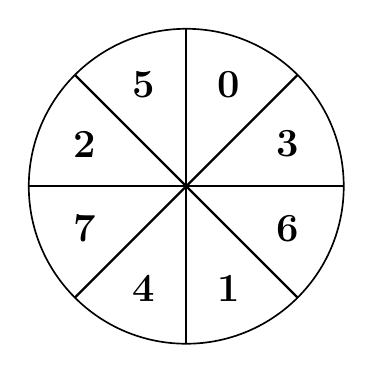
\begin{tikzpicture}
        \def\R{2cm}          
        \def\list{0,3,6,1,4,7,2,5}  
        \draw[line width=.6pt] (0,0) circle (\R);
        \foreach \idx [count=\i from 0] in \list{
            \draw[thick] (0,0) -- ++(90-\i*45:\R);
            \node at (90-\i*45-22.5:0.7*\R) {\Large\bfseries \idx};
        }
    \end{tikzpicture}
    \end{center}
\end{enumerate}

\ifx\allfiles\undefined
\end{document}
\fi